\begin{figure}[h!]
	\centering
	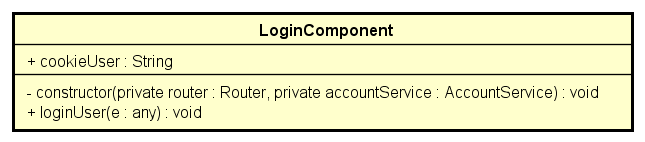
\includegraphics[scale=0.8]{res/sections/SpecificaFrontEnd/Components/Disegnetti/login.png}
	\caption{Diagramma della classe LoginComponent}
\end{figure}

\begin{itemize}
	\item \textbf{Descrizione:}\\
	È il componente che descrive la pagina di login dell’applicazione, mette a disposizione dell’utente un form dove inserire username e password. Gestisce le operazioni e la logica applicativa per il login.
	\item \textbf{Utilizzo:}\\
	Questo componente viene istanziato dinamicamente dal servizio Router del framework Angular quando viene richiesta la pagina di login.
	\item \textbf{Attributi:}
		\begin{itemize}
			\item \emph{+cookieUser: String}\\
			Riceve l'username dai cookie di sessione
		\end{itemize}
	\item \textbf{Metodi:}
		\begin{itemize}
			\item \emph{-constructor(private router: Router, private accountService: AccountService)}\\
    		Crea un istanziazione di RegistrationComponent\\
    		\textbf{Parametri:}
    		\begin{itemize}
    			\item \emph{-router: Router}
    			Necessario per l'importaziine del Router
    			\item \emph{-accountService: AccountService}
    			Necessario per l'importazione di AccountService
    		\end{itemize}
    		\item \emph{+loginUser(e: any)}\\
    		Effettua l'autenticazione dell'utente\\
    		\textbf{Parametri:}
    		\begin{itemize}
    			\item \emph{+e: any}
    			Contiente i dati dell'utente da autenticare
    		\end{itemize}
		\end{itemize}
\end{itemize}